\lhead{\begin{tikzpicture}[remember picture, overlay]
\node [anchor=100,inner sep=0] (imagenIZQUIERDA) at (current page header area.north){
\includegraphics[width=18cm]{img/Encabezado.PNG}};
\end{tikzpicture}}
\rhead{Ángeles-Hurtado}
\rfoot{\begin{tikzpicture}[remember picture, overlay]
\node [anchor=140,inner sep=0] (imagenDERECHA) at (current page footer area.south){
\includegraphics[width=18cm]{img/Foot.PNG}};
\end{tikzpicture}}
%----------------------------------------------------------------------------------------
\lfoot{ \thepage}
% \renewcommand{\labelenumi}{\alph{enumi}.)} 
%----------------------------------------------------------------------------------------
%----------------------------------------------------------------------------------------
%	TITLE SECTION
%----------------------------------------------------------------------------------------

\setlength{\droptitle}{-5\baselineskip} % Move the title up
\title{\textbf{Estudio de tiempos y movimientos en el ensamble de un circuito electrónico utilizando diferentes métodos para su optimización }} % Article title

 \author{ 
 \textsc{Fentanes Hernandez, Ana Karen}\\ 
%  Afiliación:
 \texttt{Instituto Tecnológico De Queretaro} \\ 
 \texttt{Tecnologico Nacional De Mexico } \\ 
 \texttt{Queretaro, Mexico}\\ 
 \texttt{l22140957@queretaro.tecnm.mx} 
 \and 
 \textsc{Ángeles-Hurtado, Luis Alberto}\\ 
%  Afiliación:
 \texttt{ Instituto Tecnológico de Querétaro } \\ 
 \texttt{ Tecnológico Nacional de México } \\ 
 \texttt{Querétaro, México}\\ 
 \texttt{alb3rt0.ah@gmail.com} 
}


%----------------------------------------------------------------------------------------

% \begin{document}

% Print the title
\maketitle
\thispagestyle{fancy}

%----------------------------------------------------------------------------------------
%	ARTICLE CONTENTS
%----------------------------------------------------------------------------------------

% \section*{Resumen}
% \textit{Palabras clave:}
% El resumen (ancho de página) deberá contener entre 100 y 200 palabras tipo Adobe Devangari 11 puntos.

\begin{abstract}
\noindent 
El resumen (ancho de página) deberá contener entre 100 y 200 palabras tipo Adobe Devangari 11 puntos.

\end{abstract}
% 
% 
\textbf{\textit{Palabras clave}}: {First keyword should be the corresponding to the research area according with the authors guide. Maximum of 6 keywords.}
% \keywords{First keyword should be the corresponding to the research area according with the authors guide. Maximum of 6 keywords.}

\section{Introducción}

% Define estudio de tiempos y movimientos: Es el analisis de metodos, materiales, herramientas eh innstalacion utilizado o que se ah de utilizar la ejecucuion de un trabajo 
% Define que es ensamble: Es unir, juntar, ajustar.
% Define que es circuito electronico: Es un conjunto  de elementos electricos conectados entre si que permiten general transportar y utilizar la energia. 
% Define el metodo de tiempos predeterminados: Es la reunion de tiempos estandarares validos asignados a movimientos funfamentales para el estudio del tiempo. 
% Define optimización: Es la accion de desarollar una actividad lo mas eficientemente posible.
\begin{itemize}
    \item Con base a la materia estudio del trabajo II,   este proceso implicara analizar y medir desde la colocación de componentes hasta la soldadura y prueba de circuito.  
    \item Ejecutaremos los  métodos para  identificar los tiempos que se dedicaran a cada uno de las operaciones, al igual que el estudio de tiempos y movimientos para medir el tiempo que se lograra con el circuito. 
    \item Se determinara la 
 eficiencia y técnicas del analista para optimizar el tiempo estándar de cada movimiento y proceso ,mas adelante se mencionaran los elementos, herramientas,  procesos y materiales para la plantación necesaria de estudio de tiempos y movimientos.
 
\item Estudio: Pone el entendimiento aplicándose a conocer algo.
\item Tiempo: Duración de las cosas sujetas a mudanza.
\item Movimiento: Acción y efecto de mover.
\item Circuito: Terreno comprendido dentro de un perímetro cualquiera.
\item Electrónico: Proceso de la unión de dos partes.
\item Optimización: Acción y efecto de optimizar.
\end{itemize}
% 
% 
\section{Justificación}

\begin{itemize}
    \item Lo que se requiere es identificar y eliminar posibles errores, se utilizaran diferentes  métodos para maximizar el tiempo estándar y así lograr un mejor resultado.  
    \item Debe de tener Referencias científicas, URL, tesis, etc.
\end{itemize}
% 
% 
\section{Descripción del problema}
\begin{itemize}
    \item Es un proceso que debe ser mejorado para la facilidad del operario y analista, logrando un resultado eficaz y complejo, tomando en cuenta el calculo del tiempo y analizar los datos de ese mismo.
    \item Es eficiente utilizar diferentes métodos, serán diferentes variables las que se necesitan ejecutar para saber cual de todos los procesos es el que mejor nos conviene para la fabricación del ensamble del circuito para ello se planteara la tabla Bimanual. 
    \item Debe de tener Referencias científicas, URL, tesis, etc.
\end{itemize}

\textbf{*La incógnita científica es el elemento cuya solución incrementa el conocimiento científico.}
% 
% 
\section{Fundamentación teórica}

Con base a las técnicas que se emplean en la medición del trabajo la más importante es el estudio de tiempos la cual sera realizada para la medición y planificación de este circuito.
\begin{itemize}
    \item Teorema: Proposición demostrable lógicamente partiendo de axiomas, postulados o de otra proposición.
    \cite{TEOREMA-2022} 
    \item Proposición: Enunciación de una verdad demostrada o que se trata de demostrar.
    \item Axioma: Proposición tan clara y evidente que se admite sin demostración.
    \cite{AXIOMA-2023}
    \item Enunciar: Exponer el conjunto de datos de un problema.
    \cite{Enunciado-2023}
    \item Estudio de Movimientos: Análisis detallado de los movimientos individuales
    que componen una tarea para identificar mejoras en eficiencia.
    \item El analista: se encarga de recopilar datos e información relevante para tomar decisiones informadas sobre inversiones, riesgos y oportunidades en los mercados.
    \item Referencias solo de artículos y libros científicos.
\end{itemize}
% 
%
\begin{itemize}
\section{Hipótesis}

    
\item  Se debe de identificar claramente el fundamento

\item  Se debe identificar claramente la variable de respues-
gracias
Se debe identifican claramente las realidades o mo-
delos contrastantes
Se debe de establecer las variables asociadas, 
\end{itemize}
% 
%
\begin{itemize}
    \section{Objetivo}
    
\item Determinar mediante los objetivos Históricos el tiempo producto con otros métodos. 
 \item Diseño, implementar y mejorar sistemas productivos aplicando tecnologías para su optimización y elevar la productividad. 
\end{itemize}


\subsection{Objetivos específicos }

\begin{itemize}
    \item Realizar los ensambles requeridos para el funcionamiento adecuado.
    \item Identificar las técnicas y herramientas utilizadas en el estudio de tiempos y movimientos en el ensamble.
    \item Analizar la importancia  para la mejora continua de la eficiencia.
    \item Reconocer todos los movimientos de cada pieza que sera empleada en el proceso.
    \item Aplicar de manera correcta los métodos establecidos.
\end{itemize}

Son actividades orientadas al cumplimiento del objetivo general. Se establecen con verbos activos en infinitivo. Son parte de la acción encaminada a probar la hipótesis. Éstos deben ser precisos, y en lo posible evitar aspectos metodológicos.
% 
% 
\section{Cuerpo (Metodología, modelo matemático, etc.)}

Se tiene como objetivo el determinar mediante los registros históricos y aplicar los conocimientos adquiridos y saber el manejo y calculo del tiempo para un mejor panorama  y los proceso adecuados para la optimización del tiempo

\begin{table}[H]

    \huge
    \tiny
    \begin{tabular}{|c|c|c|}
    
    \hline
    NOMBRE & PIEZA & PLANO\\
    \hline
    CABLE MH & \includegraphics[width=12mm]{9/Img/PIEZACableMH.PDF}\ref{anexo:PIEZACABLEMH} & \includegraphics[width=12mm]{9/Img/PLANOCableMh.pdf}\ref{anexo:PLANO.CABLEMH}\\
    \hline
    CABLE MM & \includegraphics[width=12mm]{9/Img/PIEZACableMM.PDF}\ref{anexo:PIEZACABLEMM} & \includegraphics[width=12mm]{9/Img/PLANOCableMm.pdf}\ref{anexo:PLANOCABLEMM}\\
    \hline
    RESISTENCIA &\includegraphics[width=12mm]{9/Img/PIEZAResistencia.pdf}\ref{anexo:PIEZARESISTENCIA} & \includegraphics[width=12mm]{9/Img/PLANOResistencia.pdf}\ref{anexo:PLANORESISTENCIA}\\
    \hline
    LCD &  \includegraphics[width=12mm]{9/Img/PIEZALcd.pdf}\ref{anexo:PIEZALCD} & \includegraphics[width=12mm]{9/Img/PLANOLcd.PDF}\ref{anexo:PLANOLCD}\\
    \hline
    ESP & \includegraphics[width=12mm]{9/Img/PIEZAEsp32.pdf}\ref{anexo:PIEZAESP32} & \includegraphics[width=12mm]{9/Img/PLANOEsp32.PDF}\ref{anexo:PLANOESP32}\\
    \hline
    POTENCIOMETRO & \includegraphics[width=12mm]{9/Img/PIEZAPotenciometro.pdf}\ref{anexo:PIEZAPOTENCIOMETRO} & \includegraphics[width=12mm]{9/Img/PLANOPotenciometro.pdf}\ref{anexo:PLANOPOTENCIOMETRO}\\
    

    \end{tabular}
    \caption{PIEZAS SOLIDWOKS}
    \label{tab:my_label}
\end{table}[1]
% 
% 


Antes de que comiences a utilizar esta plantilla, es recomendable que prepare la información que contendrá en un archivo aparte. 
Ten preparadas tus gráficas, así como también las tablas aparte, para que sea más fácil integrarlo.  
Se recomienda fuertemente el uso de \textbf{formato Enhanced Metafile (.emf) para imágenes y gráficas} de resolución óptima. 
Finalmente, completa y organiza el contenido antes de darle el formato de esta plantilla. 

\subsection{Acrónimos y Abreviaciones}

Los acrónimos y abreviaciones deberán ser definidos únicamente la primera vez que aparecen en el texto, esto para que el lector entienda lo que significan.

\subsection{Ecuaciones}

Las ecuaciones son una excepción a las especificaciones prescritas de esta plantilla. 
Deberá determinar si su ecuación debe escribirse o no utilizando la fuente Adobe Devangari. 
Para crear ecuaciones multinivel, puede ser necesario tratar la ecuación como un gráfico e insertarla en el texto después de aplicar el estilo de la platilla.
Las ecuaciones serán enumeradas de manera consecutiva, y el número de ecuación, entre paréntesis, se colocan al ras de la derecha, utilizando una tabulación derecha. 

\begin{equation}
    \label{eq1}
    x + y = z 
\end{equation}

Es importante asegurarse de que los símbolos de la ecuación sean definidos antes o inmediatamente después de la ecuación. Utilice “(1)”, en vez de “Eq. 1” al enumerar las ecuaciones, excepto al principio de una oración: “La ecuación (\ref{eq1}) es”



\section{Resultados y discusión}

Antes de comenzar a preparar tu artículo, es importante que lea primero la guía del autor, la cual incluye los temas o apartados que son necesarios para tener tu trabajo completo.
Una vez completada la edición del texto, el documento está listo para el uso de esta plantilla. En este archivo recién creado, resalte todo el contenido e importe el archivo de texto preparado. Ahora esta listo para estilizar su documento.
En esta sección se deben presentar todo lo obtenido de la sección 2, incluidas deducciones o efectos del desarrollo. También se podrán incluir bisecciones numeradas de la siguiente forma:

\subsection{Autores y Afiliaciones}

Para distinguir las afiliaciones de los autores, utilice superíndices iniciando con el número 1, 2, etc., sucesivamente, esto dependerá de la cantidad de los departamentos a los que estén afiliados los autores. En caso de que todos los autores pertenezcan a una mismo departamento e institución, utilizar sólo el superíndice 1. 
+c
\subsection{Identificar los encabezados}

Se les recuerda a los autores que los encabezados deben de estar conforme los solicita la guía del autor. De ahí se puede adaptar el trabajo para que sea más fácil de entender para el lector.
Los encabezados organizan los temas sobre una base relacional y jerárquica. Por ejemplo, el título del documento es encabezado del texto principal porque todo el material posterior se relaciona y elabora sobre este tema. 

\subsection{Tablas y Figuras}

\begin{enumerate}


    \item Posición de las tablas y figuras: Coloque las figuras y las tablas en la parte superior e inferior de las columnas. Evite colocarlos en medio. Las figuras y las tablas grandes pueden abarcar ambas columnas. Los títulos de las figuras deben de estar debajo de las mismas; los títulos de las tablas deben aparecer encima de ellas. Insértese las figuras y los cuadros después de citarse en el texto. Utilice la abreviatura “Fig. 1”, incluso al principio de una oración. 
\end{enumerate}

\section{Conclusiones}

Se describe aquí el alcance del trabajo, logros obtenidos y perspectivas para el futuro de este. Se sugiere colocar información cuantitativa obtenida.

\section{Agradecimientos}

Es importante darles su debido reconocimiento a los laboratorios, instituciones, organizaciones, entre otros que han sido participes para la culminación de este trabajo. También es importante mencionar, fondos, proyectos, becas, entre otros que se le han otorgado al o los autores para realizar el trabajo de investigación. Ejemplo: “Los autores agradecen al Concejo Nacional de Ciencia y Tecnología por los recursos otorgados…”

\section*{Referencias}



Enumere las notas al pie por separado en superíndices. Coloque la nota de pie de en la parte inferior de la columna en la que se citó. No coloque notas al pie en la lista de referencias. Utilice letras para las notas al pie de la tabla.
A menos de que haya tres autores o más; no utilice “et al.”. Los trabajos que no hayan sido publicados, incluso si han sido presentados para su publicación, deben ser citados como “inéditos”. Los trabajos que han sido aceptados para su publicación deben de citarse como “en prensa”. Poner en mayúscula sólo la primera palabra de un título, excepto los nombres propios y los símbolos de elemento. 
% Otros ejemplos \cite{LAAngeles2021}, \cite{LAAngelesConni}. 
%Véase el link \cite{prueba}.



% Ejemplo
%  @Article{article,
% 	author = "Author1 LastName1 and Author2 LastName2 and Author3 LastName3",
% 	title = "Article Title",
% 	volume = "30",
% 	number = "30",
% 	pages = "10127-10134",
% 	year = "2013",
% 	doi = "10.3389/fnins.2013.12345",
% 	URL = "http://www.frontiersin.org/Journal/10.3389/fnins.2013.12345/abstract",
% 	journal = "Frontiers in Neuroscience"
% }

% @book{book,
%   author    = {Author Name}, 
%   title     = {The title of the work},
%   publisher = {The name of the publisher},
%   address   = {The city},
%   year      = 1993,
% }

% @incollection{chapter,
%   author       = {Bauthor Surname}, 
%   title        = {The title of the work},
%   editor       = {Editor Name},
%   booktitle    = {The title of the book},
%   publisher    = {The name of the publisher},
%   address      = {The city},
%   year         = 2002,
%   pages        = {201-213},
% }

% @InProceedings{conference,
%   author = {Cauthor Name and Dauthor Surname and Fauthor LastName},
%   title = {The title of the work},
%   booktitle = {The title of the conference proceedings},
%   year = 1996,
%   publisher = {The name of the publisher},
%   editor = {Editor Name1 and Editor Name2},
%   pages = {41-50},
% }

% @book{cho,
%   author       = {Gauthor Name1}, 
%   title        = {The title of the work},
%   publisher = {Country code and patent number},
%   address      = {Patent Country},
%   year = 2013
% }

% @book{patent,
%   author    = {Hauthor Surname1}, 
%   title     = {The title of the work},
%   publisher = {Patent number},
%   address   = {Patent country},
%   year      = 2010,
% }

% % please use misc for datasets
% @misc{dataset, 
% 	author = "Author1 LastName1 and Author2 LastName2 and Author3 LastName3",
% 	title = "Data Title",
% 	year = "2011",
% 	doi = "10.000/55555",
% 	URL = "http://www.frontiersin.org/",
% }

\bibliographystyle{ieeetr}
\bibliography{9/referencias}
% 
% 
%%%%%%%%%%%%%%%%%%%%%%%%%%%%%%%%%%
\appendix
%%%%%%c%%%%%%%%%%%%%%%%%%%%%%%%%%%%
% 
\newpage
\centering{\section[\appendixautorefname{}]{Apéndice}}\label{anexo:MANUAL}
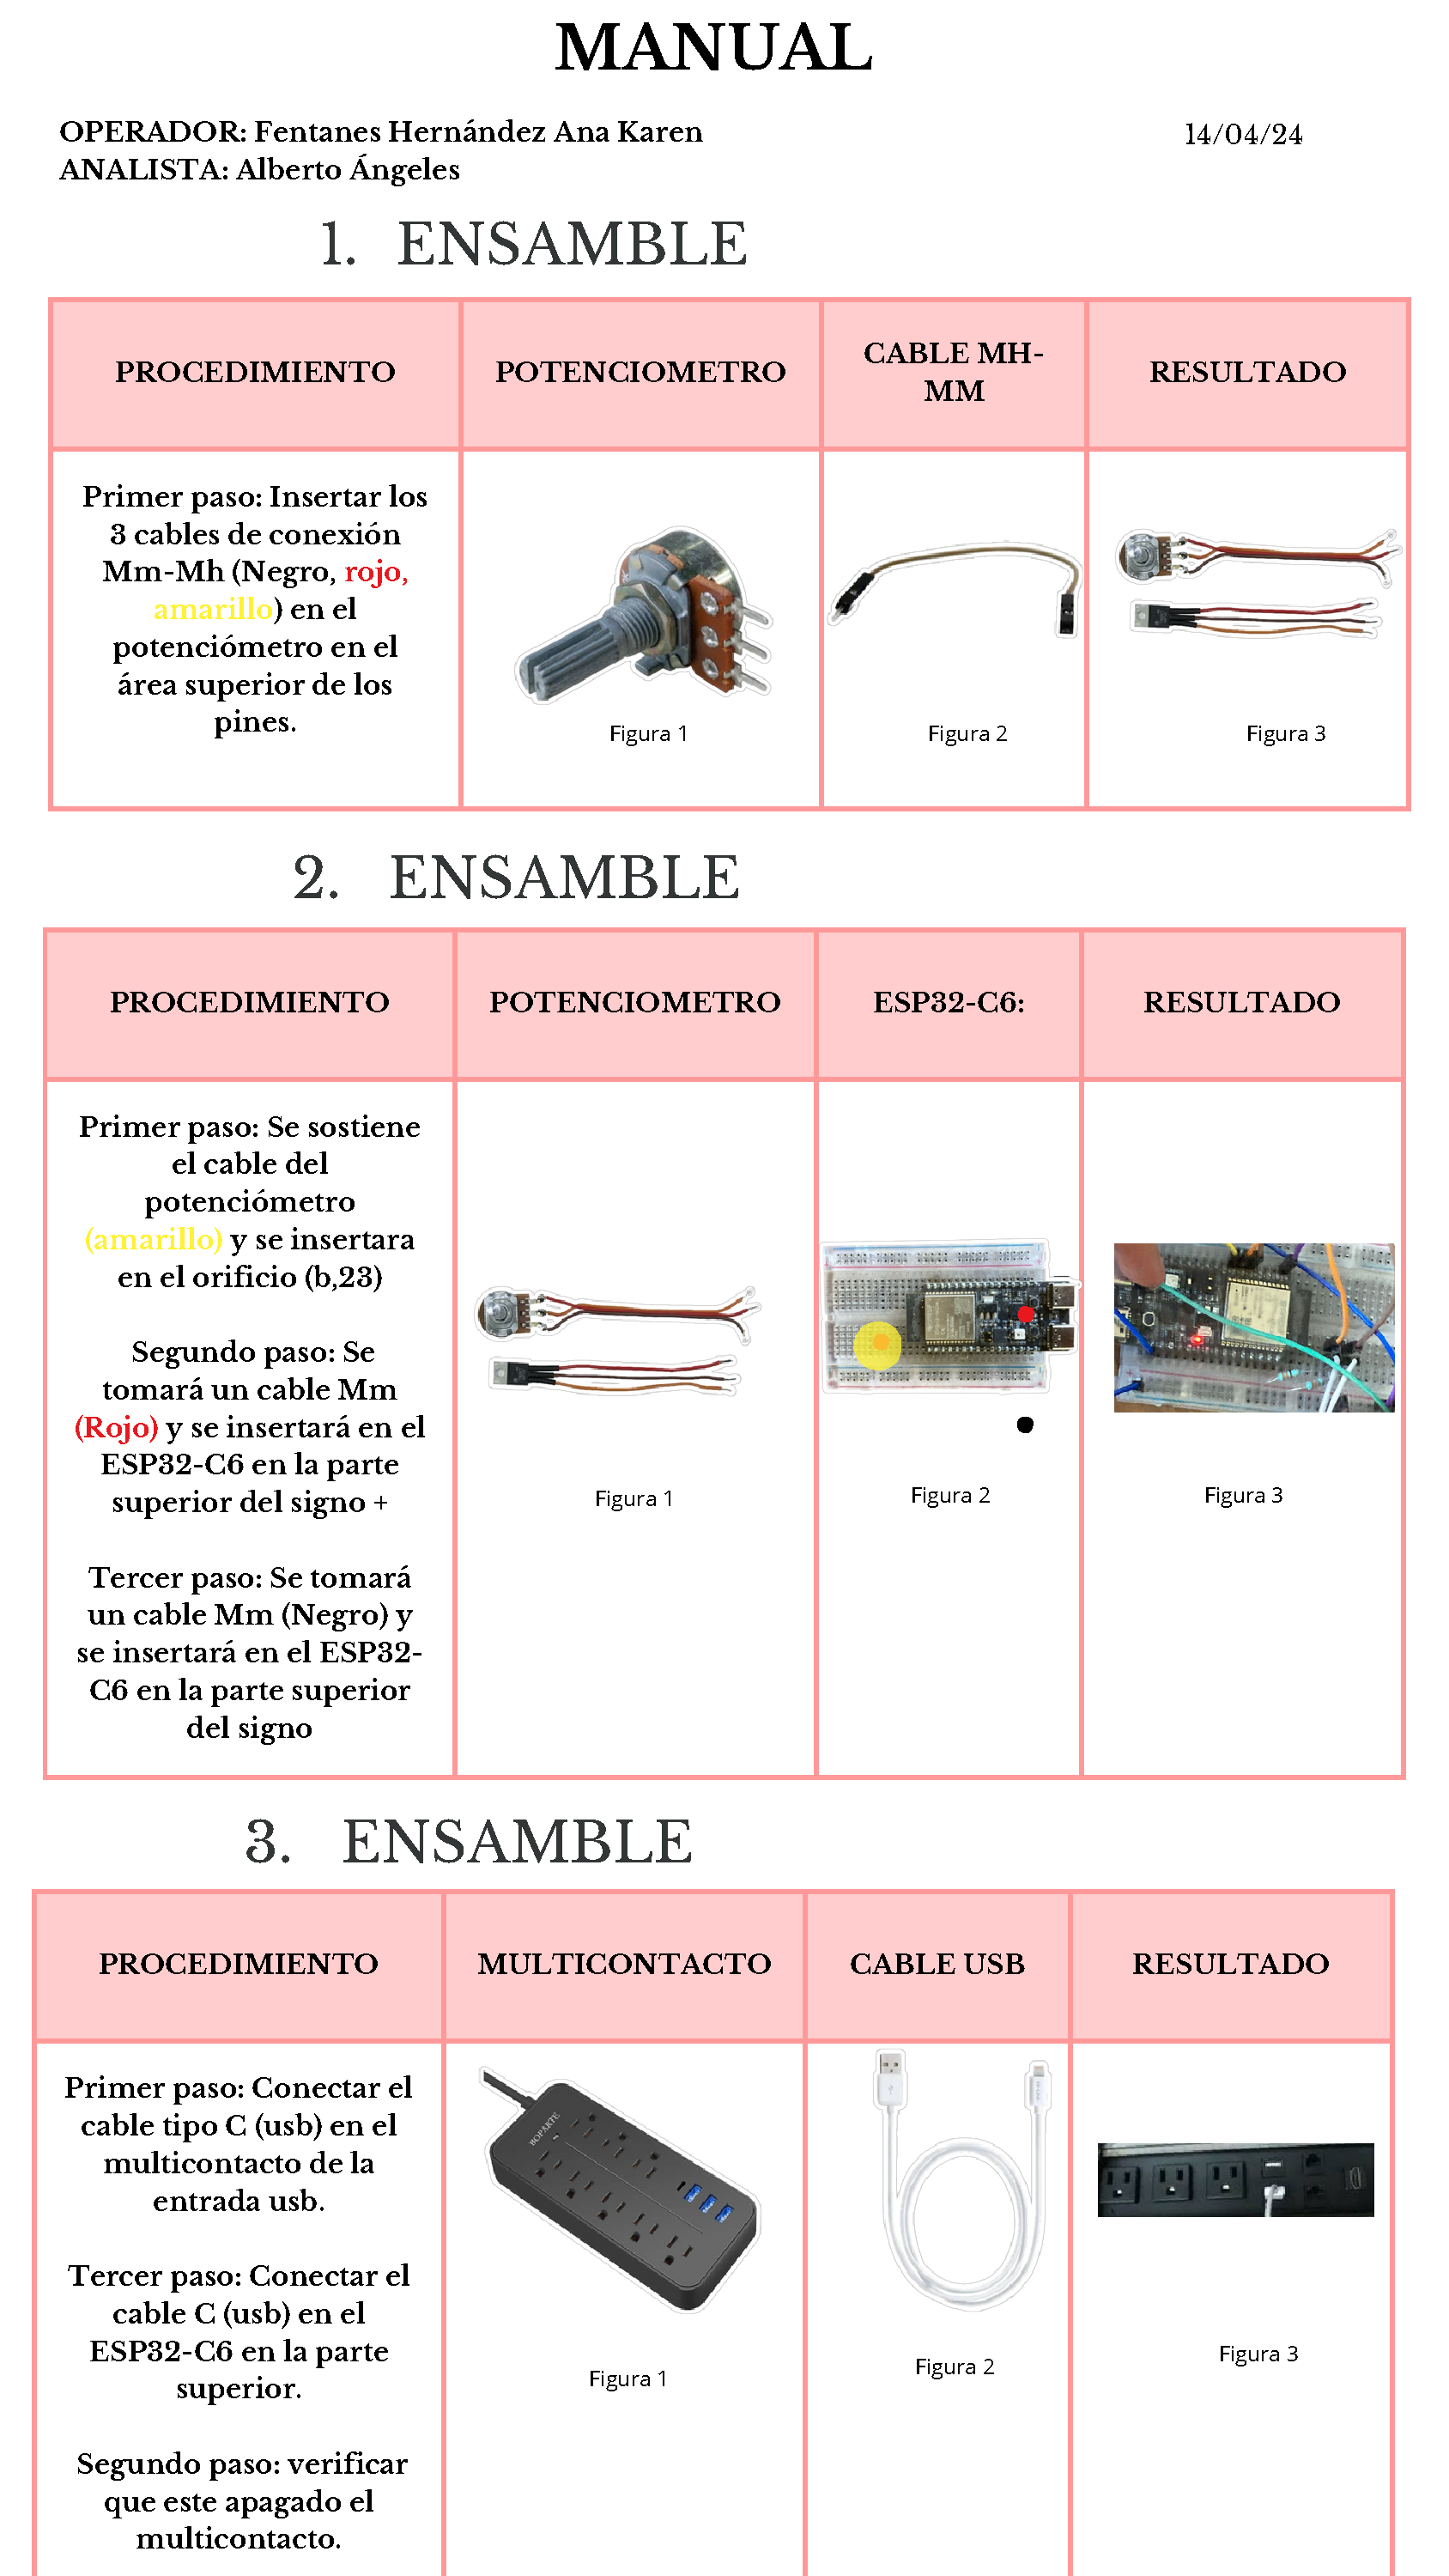
\includepdf[pages=-]{9/Img/MANUAL ENSAMBLE.pdf}
%
\newpage
\centering{\section[\appendixautorefname{}]{Apéndice}}\label{anexo:REGISTRO}
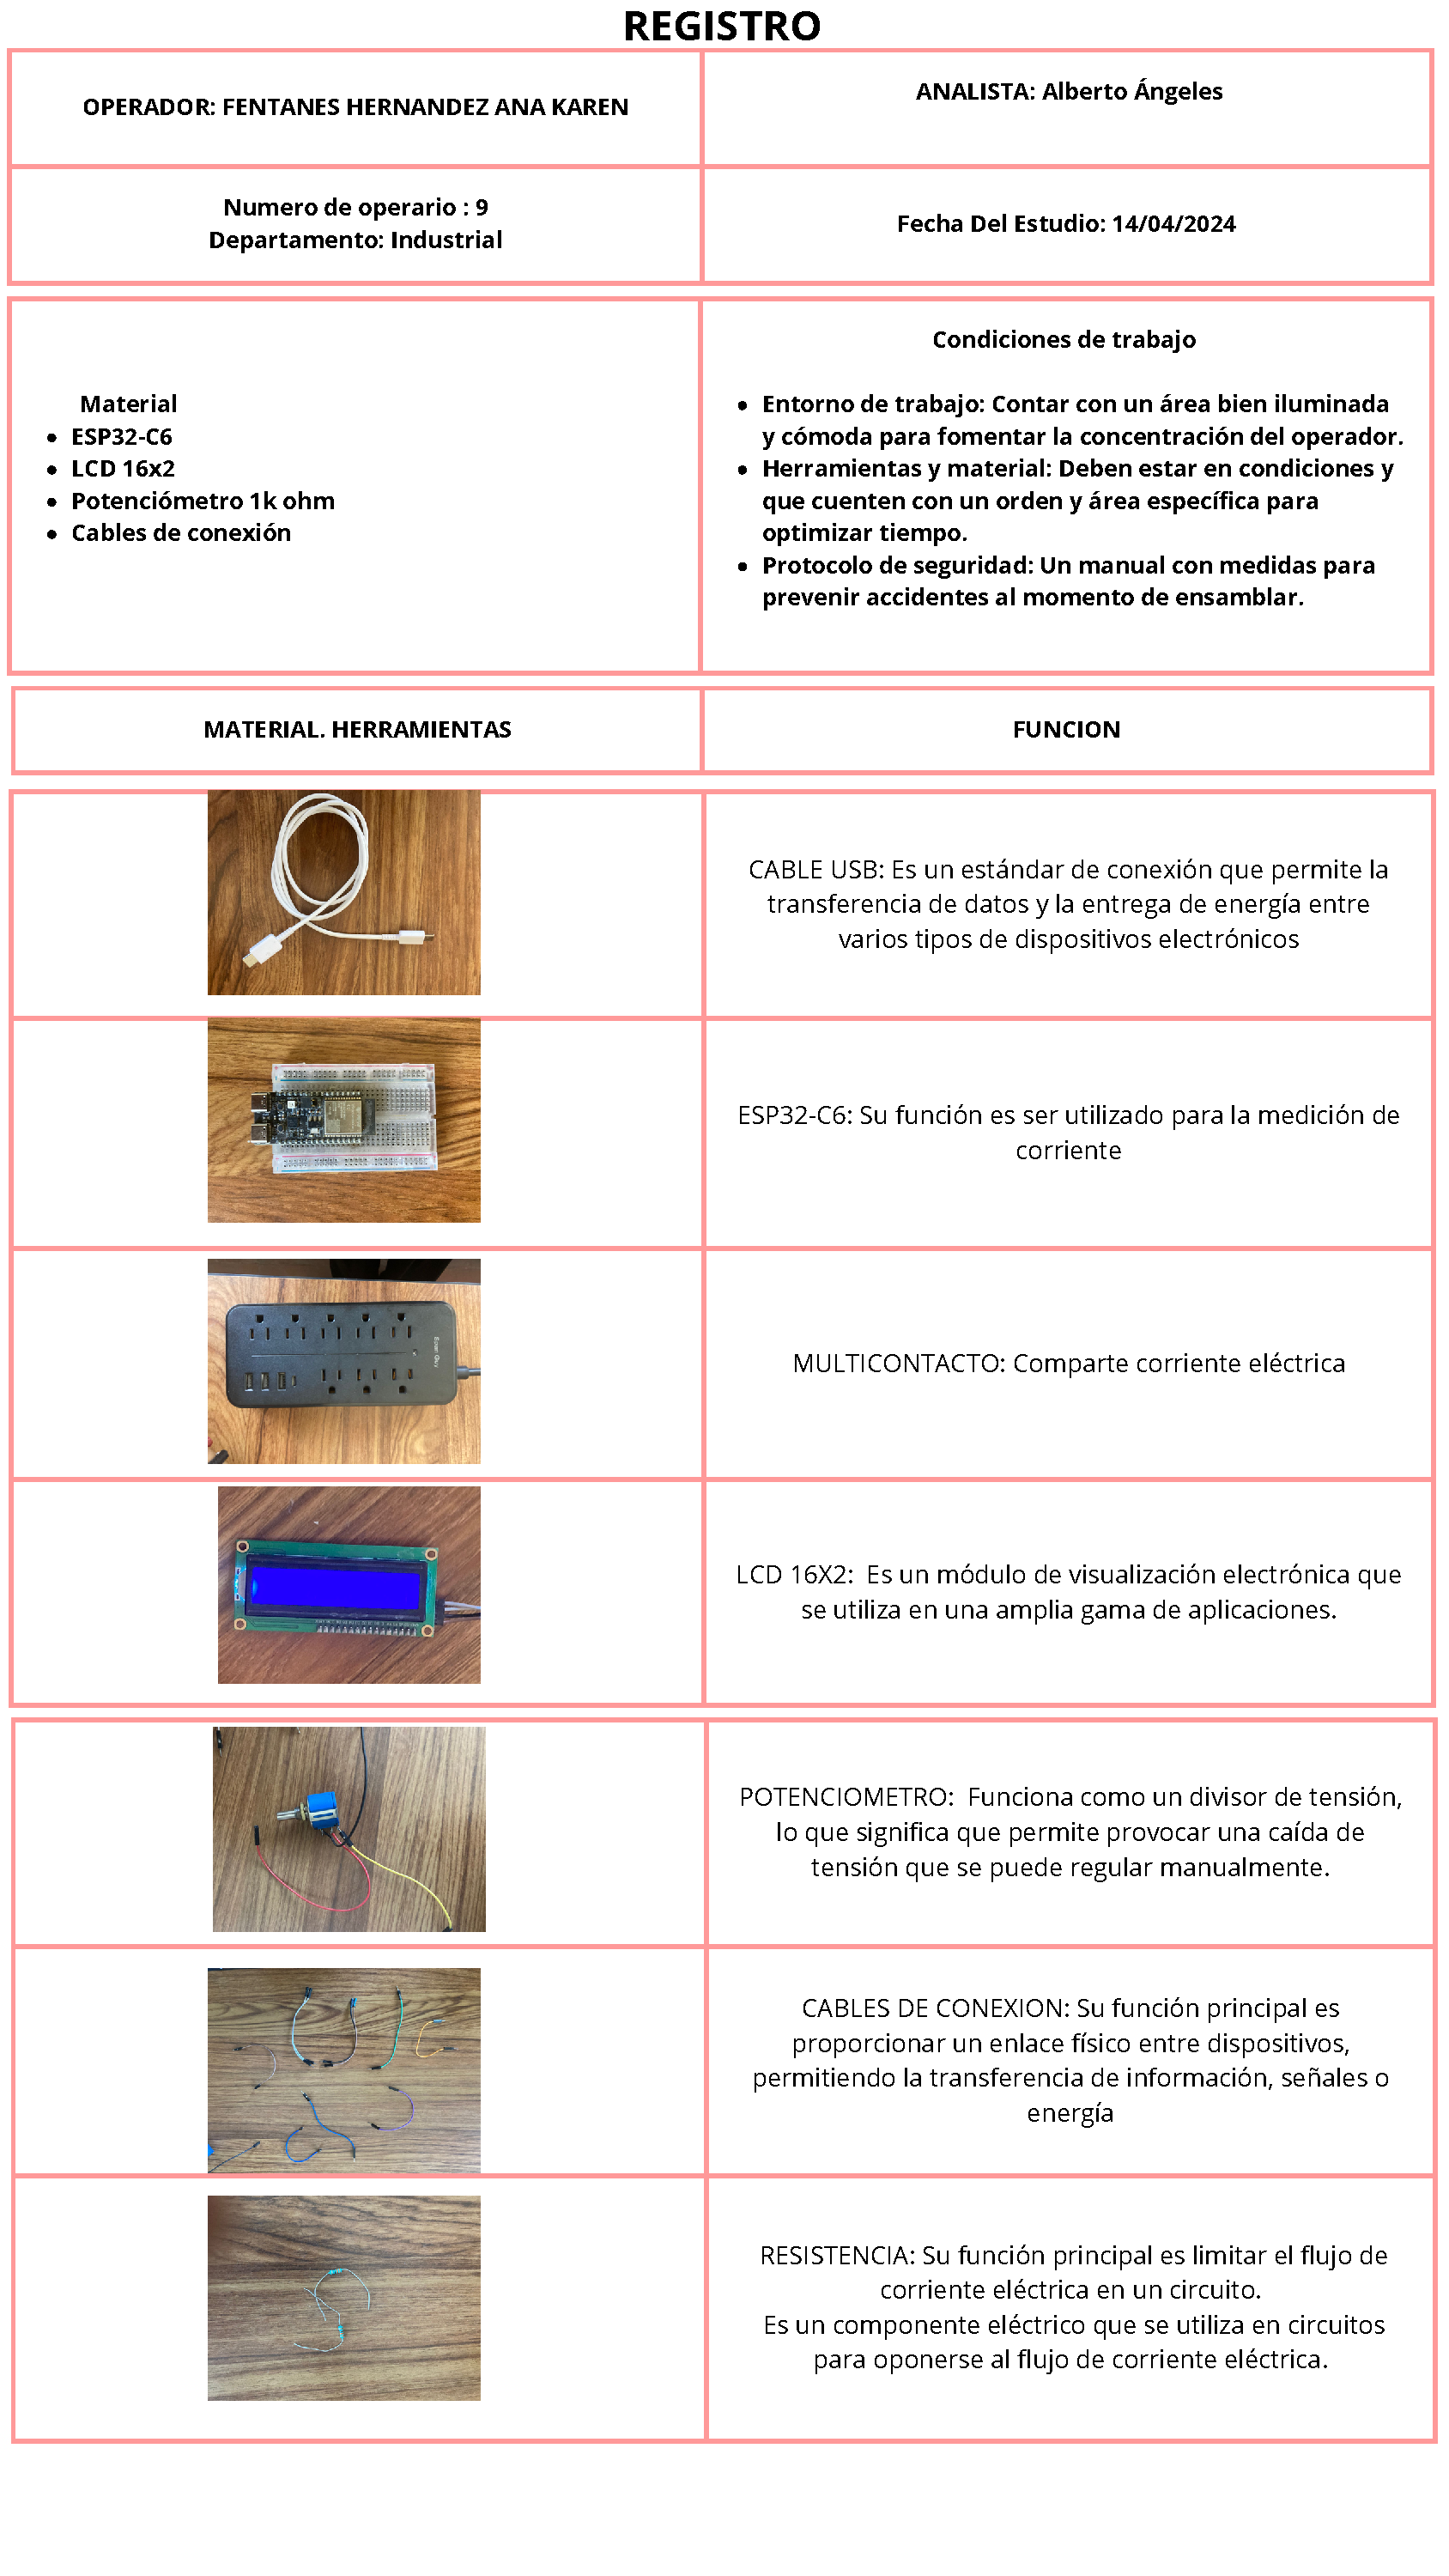
\includepdf[pages=-]{9/Img/REGISTRO.pdf}
%
\newpage
\centering{\section[\appendixautorefname{}]{Apéndice}}\label{anexo:PLANOCABLEMM}
\includepdf[pages=-]{9/Img/PLANOCableMm.pdf}
%
\newpage
\centering{\section[\appendixautorefname{}]{Apéndice}}\label{anexo:PLANO.CABLEMH}
\includepdf[pages=-]{9/Img/PLANOCableMh.pdf}
%
\newpage
\centering{\section[\appendixautorefname{}]{Apéndice}}\label{anexo:PLANORESISTENCIA}
\includepdf[pages=-]{9/Img/PLANOResistencia.pdf}
%
\newpage
\centering{\section[\appendixautorefname{}]{Apéndice}}\label{anexo:PLANOLCD}
\includepdf[pages=-]{9/Img/PLANOLcd.PDF}
%
\newpage
\centering{\section[\appendixautorefname{}]{Apéndice}}\label{anexo:PLANOESP32}
\includepdf[pages=-]{9/Img/PLANOEsp32.PDF}
%
\newpage
\centering{\section[\appendixautorefname{}]{Apéndice}}\label{anexo:PLANOPOTENCIOMETRO}
\includepdf[pages=-]{9/Img/PLANOPotenciometro.pdf}
%
\newpage
\centering{\section[\appendixautorefname{}]{Apéndice}}\label{anexo:PIEZACABLEMM}
\includepdf[pages=-]{9/Img/PIEZACableMM.PDF}
%
\newpage
\centering{\section[\appendixautorefname{}]{Apéndice}}\label{anexo:PIEZARESISTENCIA}
\includepdf[pages=-]{9/Img/PIEZAResistencia.pdf}
%
\newpage
\centering{\section[\appendixautorefname{}]{Apéndice}}\label{anexo:PIEZALCD}
\includepdf[pages=-]{9/Img/PIEZALcd.pdf}
%
\newpage
\centering{\section[\appendixautorefname{}]{Apéndice}}\label{anexo:PIEZAESP32}
\includepdf[pages=-]{9/Img/PIEZAEsp32.pdf}
%
\newpage
\centering{\section[\appendixautorefname{}]{Apéndice}}\label{anexo:PIEZAPOTENCIOMETRO}
\includepdf[pages=-]{9/Img/PIEZAPotenciometro.pdf}
%
\newpage
\centering{\section[\appendixautorefname{}]{Apéndice}}\label{anexo:PIEZACABLEMH}
\includepdf[pages=-]{9/Img/PIEZACableMH}
%
\newpage
\centering{\section[\appendixautorefname{}]{Apéndice}}\label{anexo: PIEZACABLEMH}
\includepdf[pages=-]{9/Img/PIEZACableMH}
%

%%%%%%%%%%%%%%%%%%%%%%%%%%%%%%%%%%%%%%%%